\documentclass[13pt]{beamer}
%
% Choose how your presentation looks.
%
% For more themes, color themes and font themes, see:
% http://deic.uab.es/~iblanes/beamer_gallery/index_by_theme.html
%
\mode<presentation>
{
  \usetheme{CambridgeUS}     % or try Darmstadt, Madrid, Warsaw, ...
  \usecolortheme{beaver} % or try albatross, beaver, crane, ...
  \usefonttheme{default}  % or try serif, structurebold, ...
  \setbeamertemplate{navigation symbols}{}
  \setbeamertemplate{caption}[numbered]
} 

\usepackage[english]{babel}
\usepackage[utf8x]{inputenc}
\usepackage{xcolor}
\usepackage{multicol}
\usepackage{tikz}
\usepackage{tikz-uml}
%\usepackage{pgf-umlcd}
\usepackage{graphicx}
\graphicspath{ {./images/} }

\usepackage{listings}
\definecolor{codegreen}{rgb}{0,0.6,0}
\definecolor{codegray}{rgb}{0.5,0.5,0.5}
\definecolor{codepurple}{rgb}{0.58,0,0.82}
\definecolor{backcolour}{rgb}{0.95,0.95,0.92}

\lstdefinestyle{mystyle}{
    backgroundcolor=\color{backcolour},   
    commentstyle=\color{codegreen},
    keywordstyle=\color{magenta},
    numberstyle=\tiny\color{codegray},
    stringstyle=\color{codepurple},
    basicstyle=\ttfamily\footnotesize,
    breakatwhitespace=false,         
    breaklines=true,                 
    captionpos=b,                    
    keepspaces=true,                 
    numbers=left,                    
    numbersep=5pt,                  
    showspaces=false,                
    showstringspaces=false,
    showtabs=false,                  
    tabsize=1
}

\lstset{style=mystyle}

\usepackage{graphicx}
\graphicspath{ {./images/} }

\usepackage{tikz}
\usetikzlibrary{decorations.text}
\usetikzlibrary{shapes.geometric, arrows, positioning, calc, matrix}

\tikzset{
  basic box/.style={
    shape=rectangle, rounded corners, align=center,
    draw=#1, fill=#1!25},
  header node/.style={
    Minimum Width=header nodes,
    font=\strut\Large\ttfamily,
    text depth=+0pt,
    fill=white, draw},
  header/.style={%
    inner ysep=+1.5em,
    append after command={
      \pgfextra{\let\TikZlastnode\tikzlastnode}
      node [header node] (header-\TikZlastnode) at (\TikZlastnode.north) {#1}
      node [span=(\TikZlastnode)(header-\TikZlastnode)] at (fit bounding box) (h-\TikZlastnode) {}
    }
  },
  hv/.style={to path={-|(\tikztotarget)\tikztonodes}},
  vh/.style={to path={|-(\tikztotarget)\tikztonodes}},
  fat blue line/.style={ultra thick, blue}
}

\definecolor{mygray}{RGB}{208,208,208}
\definecolor{mymagenta}{RGB}{226,0,116}
\newcommand*{\mytextstyle}{\sffamily\Large\bfseries\color{black!85}}
\newcommand{\arcarrow}[3]{%
   % inner radius, middle radius, outer radius, start angle,
   % end angle, tip protusion angle, options, text
   \pgfmathsetmacro{\rin}{1.7}
   \pgfmathsetmacro{\rmid}{2.2}
   \pgfmathsetmacro{\rout}{2.7}
   \pgfmathsetmacro{\astart}{#1}
   \pgfmathsetmacro{\aend}{#2}
   \pgfmathsetmacro{\atip}{5}
   \fill[mygray, very thick] (\astart+\atip:\rin)
                         arc (\astart+\atip:\aend:\rin)
      -- (\aend-\atip:\rmid)
      -- (\aend:\rout)   arc (\aend:\astart+\atip:\rout)
      -- (\astart:\rmid) -- cycle;
   \path[
      decoration = {
         text along path,
         text = {|\mytextstyle|#3},
         text align = {align = center},
         raise = -1.0ex
      },
      decorate
   ](\astart+\atip:\rmid) arc (\astart+\atip:\aend+\atip:\rmid);
}
\title[Design Pattern]{Creational Design Pattern}
\author{Hung Tran}
\institute{Fpt software}
\date{\today}


\begin{document}

\begin{frame}
  \titlepage
\end{frame}

% Uncomment these lines for an automatically generated outline.
\begin{frame}{Outline}
  \tableofcontents
\end{frame}

\section{Introduction}

\begin{frame}{Design Pattern}

\begin{columns}[T]
\begin{column}{.5\textwidth}                                          
	\begin{itemize}
		\setlength\itemsep{1em}  
		\item Published in 1995.
		\item Known as gang of four design pattern.
		\item Describes solutions to common object oriented design problems.
		\item Examples in small talk and C++.
		\item Implemented directly in some languages.
	\end{itemize}                                
\end{column}

\begin{column}{.5\textwidth}                                              
	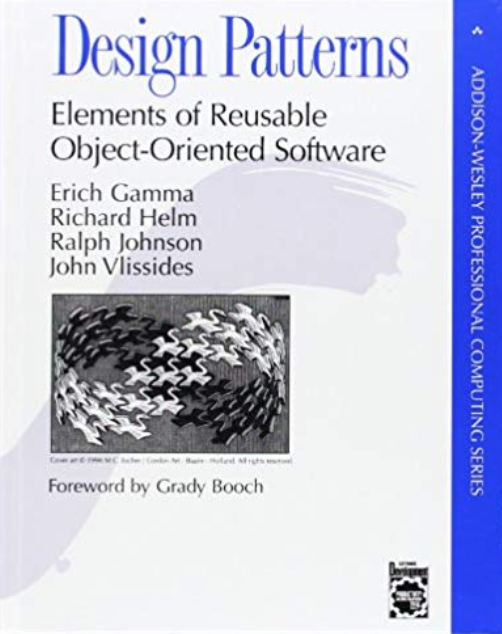
\includegraphics[scale=0.3]{gangoffour.png}
\end{column}%
\end{columns}
\end{frame}

\begin{frame}{What is Design Pattern?}
	\begin{itemize}
		\item Language and domain independent strategies for solving common object-oriented design 					  problems.
		\item These problems are recurring and can appear in all kinds of applications.
		\item Describes solutions to common object oriented design problems, irrespective of their 					  language or platform.
		\item Patterns provide suggestions - different ways to solve these common problems.
		\item Developers can use these suggestions as guidelines to create solution for their 						  problems.
		%\item The proposed solution can nave different implementation alternative, depending on the 					  programming language, framework or specific platform.
	\end{itemize}
\end{frame}

\begin{frame}{Classification of Design Pattern}
\begin{table}[h!]
  \begin{center}
    \caption{Design Pattern Classification}
    \begin{tabular}{|c|c|c|c|} % <-- Alignments: 1st column left, 2nd middle and 3rd right, with vertical lines in between
		\hline      
      	\textbf{Scope} & \textbf{Creational} & \textbf{Structural} & \textbf{Behavioral}\\
		\hline	  	
	  	Class & Factory Method & Adapter & Interpreter \\
	  		& 				& 		  & Template\\
	  		&				&		  & Method\\    
      	\hline
      	Object & Abstract Factory, & Adapter, & Chain of\\ 
      		 &				   & 		 & Responsibility,\\
       		 & Builder, & Bridge, & Command,\\
       		 & Prototype, & Composite, & Iterator,\\
       		 & Signleton & Decorator, & Mediator,\\
       		 & 			 & Facade, & Memento,\\
       		 &			 & Flyweight, & Observer,\\
       		 &			 & Proxy, & State, Strategy,\\
      	\hline
    \end{tabular}
  \end{center}
\end{table}
\end{frame}

\begin{frame}{Overview of UML class diagram}
	\begin{itemize}
		\item It depicts relationships between classes that make up the pattern
		\item It is important to understand class notations to understand the structure of the 				  pattern
	\end{itemize}
	
\begin{columns}[T] % align columns                                         
\begin{column}{.5\textwidth}                                               
  	\begin{center}
	\begin{tikzpicture}
	\umlclass[x=2,y=-10]{ClassName}{attribute: type \\ attribute: type}{operation \\ operation}
	\end{tikzpicture}	
	\end{center}                                                               
\end{column}%                                                              
                                                                           
\begin{column}{.5\textwidth}                                              
  	\begin{center}
	\begin{tikzpicture}
	\umlclass[x=2,y=-10]{Account}{no: int \\ name: string \\ balance: int}{GetBalance \\ Withdraw \\ Deposit}
	\end{tikzpicture}	
	\end{center}                            
\end{column}%                                                              
\hfill%                                                                    
\end{columns}
\end{frame}

\begin{frame}{Overview of UML class diagram}
	\begin{itemize}
		\item Inheritance (Generalization)
	\end{itemize}
	
	\begin{center}
	\begin{tikzpicture}
	\umlclass[x=2,y=-10]{Account}{}{}
	\umlclass[x=0,y=-12]{Savings}{}{}
	\umlclass[x=4,y=-12]{Current}{}{}
	\umlinherit[geometry=-|]{Savings}{Account}
	\umlinherit[geometry=-|]{Current}{Account}
	\end{tikzpicture}	
	\end{center}
\end{frame}

\begin{frame}{Overview of UML class diagram}
	\begin{itemize}
		\item Abstract class
	\end{itemize}
	
	\begin{center}
	\begin{tikzpicture}
	\umlclass[x=2,y=-10]{Shape}{}{\umlvirt{Draw()}}
	\umlclass[x=0,y=-12]{Line}{}{Draw()}
	\umlclass[x=4,y=-12]{Circle}{}{Draw()}
	\umlinherit[geometry=-|]{Line}{Shape}
	\umlinherit[geometry=-|]{Circle}{Shape}
	\end{tikzpicture}	
	\end{center}
\end{frame}

\begin{frame}{Overview of UML class diagram}
	\begin{itemize}
		\item Composition
	\end{itemize}
	
	\textbf{When container destroyed, all its elements destroyed}
	% Window instance owns the button
	
	\begin{center}
	\begin{tikzpicture}
	\umlclass[x=0,y=-12]{Window}{}{}
	\umlclass[x=4,y=-12]{Button}{}{}
	\umlunicompo[geometry=-|]{Button}{Window}
	
	\umlclass[x=0,y=-14]{Paragraph}{}{}
	\umlclass[x=4,y=-14]{Sentences}{}{}
	\umlunicompo[geometry=-|]{Sentences}{Paragraph}
	\end{tikzpicture}	
	\end{center}
\end{frame}

\begin{frame}{Overview of UML class diagram}
	\begin{itemize}
		\item Aggregation
	\end{itemize}
	
	\textbf{When container destroyed, its elements may not be destroyed}
	% Student may be used by other training
	% Training instance does not own the student
	% Member may joined to other team
	
	\begin{center}
	\begin{tikzpicture}
	\umlclass[x=0,y=-12]{Student}{}{}
	\umlclass[x=4,y=-12]{Training}{}{}
	\umlaggreg[geometry=-|]{Training}{Student}
	
	\umlclass[x=0,y=-14]{Passenger}{}{}
	\umlclass[x=4,y=-14]{Car}{}{}
	\umlaggreg[geometry=-|]{Car}{Passenger}
	
	\umlclass[x=0,y=-16]{Member}{}{}
	\umlclass[x=4,y=-16]{Team}{}{}
	\umlaggreg[geometry=-|]{Team}{Member}
	\end{tikzpicture}	
	\end{center}
\end{frame}

\begin{frame}{Overview of UML class diagram}
	\begin{itemize}
		\item Association
	\end{itemize}
	
	\begin{center}
	\begin{tikzpicture}
	\umlclass[x=0,y=-12]{Application}{}{}
	\umlclass[x=4,y=-12]{Data}{}{}
	\umlassoc[geometry=-|]{Application}{Data}
	
	\umlclass[x=0,y=-14]{Driver}{}{}
	\umlclass[x=4,y=-14]{Car}{}{}
	\umluniassoc[geometry=|-]{Driver}{Car}
	\end{tikzpicture}	
	\end{center}

	\begin{itemize}
		\item Note
	\end{itemize}
	
	\begin{center}
	\begin{tikzpicture}
	\umlemptyclass{A}
	\umlnote[x=3]{A}{text}
	\end{tikzpicture}
	\end{center}
\end{frame}

\begin{frame}{SOLID principles}
\begin{columns}[T]
\begin{column}{.5\textwidth}                                               
	\begin{itemize}
		\setlength\itemsep{2em}
		\item Single Responsibility Principle \\ 
		\item Open Closed Principle \\
		\item Liskov Substitution Principle \\
		\item Interface Segregation Principle \\
		\item Dependency Inversion Principle
	\end{itemize}                                
\end{column}

\begin{column}{.5\textwidth}                                              
	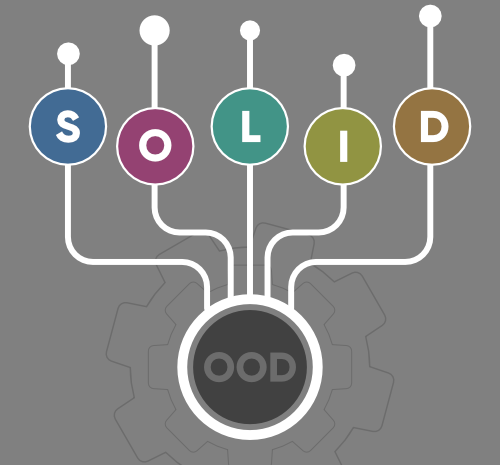
\includegraphics[scale=1]{solid.png}
\end{column}%
\end{columns}
\end{frame}

\begin{frame}{i. Single Responsibility Principle}
	\begin{center}
		\textcolor{blue}{\textbf{A class should have only one reason to change}}
	\end{center}
	\begin{itemize}
		\item Should have only one responsibility
		\item Class with multiple responsibilities break when changed
		\item Put each responsibility in a separate class
	\end{itemize}
	\textbf{Example}:                                        
% Notes class stores notes (simple text). This class only manages notes and should not responsible for display them. Notes can be displayed in any form. This implementation violates the single responsibility principle. We should separate them in different classes. 
	\begin{center}
	\tikzumlset{fill class=red!20, fill template=violet!10, font=\bfseries\footnotesize}
	\begin{tikzpicture}
	%\draw[blue, very thick] (0,0) rectangle (3,2);
	\textbf{	\umlclass[x=0,y=-12]{Notes}{}{void Add() \\ void Remove()  \\ void Display()}
	\umlnote[y=-14]{Notes}{before}
	\umlclass[x=4,y=-12]{Notes}{}{ void Add() \\ void Remove()}
	\umlclass[x=8,y=-12]{View}{}{void Display(Notes *pNotes)}}
	\umlnote[x=4,y=-14]{Notes}{after}
	\umlnote[x=8,y=-14]{View}{after}
	\end{tikzpicture}	
	\end{center}
\end{frame}

\begin{frame}{ii. Open-Closed Principle}
	\begin{center}
		\textcolor{blue}{\textbf{Modules should be open for extension but closed for 						modification}}
	\end{center}
	
	\begin{itemize}
		\setlength\itemsep{1em} 
		\item Modification to existing code leads to bugs and causes the software to break
		\item It should be possible to change behaviour of existing code without modification
		\item Instead the behaviour should be changed by adding new code
		\item Cornerstone of good design
	\end{itemize}            
% able to change behaviour in the future by adding new code. Good design is that adding new feature by adding new code not modifying existing code. (using design pattern)
	\textbf{Example}: openClosePrin.cpp
\end{frame}

\begin{frame}{iii. Liskov-Substitution Principle}
	\begin{center}
		\textcolor{blue}{\textbf{Subtypes must be substitutable for their base types}}
	\end{center}
	
	\begin{itemize}
		\setlength\itemsep{1em}
		\item Applies to inheritance relationship
		\item The inheritance relationship should be based on behavior
		\item A subclass must have all the behaviors of its base type and must not remove or change its parent behavior
		\item This allows a subclass to replace its base type in code
		\item New subclasses can be added without modifying existing code
	\end{itemize}
% Subclass should provide a different implementation of behavior compared with base class 
% This way code uses the functionality of the hierarchy to the base class will continue working if the childs pass to it.
% This allows the addition of new classes in the future
% Automatically folow open-closed principle
	\textbf{Example}: liskovsubPrin.cpp
\end{frame}

\begin{frame}{iv. Interface Segregation Principle}
	\begin{center}
		\textcolor{blue}{\textbf{Clients should not be forced to depend on methods they do not 			use}}
	\end{center}
	
	\begin{itemize}
		\setlength\itemsep{1em}
		\item An interface with too many methods will be complex to use (fat interface).
		\item Some clients may not use all the methods but will be forced to depend on them.
		\item Separate the interface and put methods based on the client usage.
	\end{itemize}
	\textbf{Example}: interfacesergregationPrin.cpp
\end{frame}

\begin{frame}{v. Dependency Inversion Principle}
	\begin{center}
		\textcolor{blue}{\textbf{Abstractions should not depend on details. Details should 				depend on abstractions}}
	\end{center}
	
	\begin{itemize}
		\setlength\itemsep{1em}
		\item Abstraction means an interface and details mean classes.
		\item Using a concrete class directly creates a dependency, software becomes difficult 			to modify.
		\item Invert the dependency by using an interface rather a concrete class.
	\end{itemize}
	\textbf{Example}: dependencyinversionPrin.cpp
\end{frame}

\begin{frame}{Creational Pattern Overview}
	\begin{center}
		\textcolor{blue}{\textbf{Construction process of an object.}}
	\end{center}
	
	\begin{itemize}
		\setlength\itemsep{1em}
		\item \textbf{Singleton}: Ensure only one instance.
		\item \textbf{Factory Method}: Create instance without depending on its concrete type.
		\item \textbf{Object pool}: Reuse existing instances.
		\item \textbf{Abstract factory}: Create instances from a specific family.
		\item \textbf{Prototype}: Clone existing objects from a prototype.
		\item \textbf{Builder}: Construct a complex object step by step.
	\end{itemize}
\end{frame}

\section{Singleton}
\begin{frame}
\textcolor{blue}{\textbf{Upcoming presentation}}
\begin{center}
\begin{tikzpicture}
\begin{umlpackage}{p}
\begin{umlpackage}{sp1}
\umlclass[y=2, template=T]{A}{n : uint \\ t : float}{}
\umlclass[y=-1]{B}{  d : double}{  \umlvirt{setB(b : B) : void} \\ getB() : B}
\end{umlpackage}
\begin{umlpackage}[x=6,y=-2]{sp2}
\umlinterface[y=1]{C}{  n : uint \\ s : string}{}
\end{umlpackage}
\umlclass[x=6,y=3]{D}{  n : uint  }{}
\end{umlpackage}
\end{tikzpicture}
\end{center}
\end{frame}
\section{Object Pool}
\begin{frame}
\textcolor{blue}{\textbf{Upcoming presentation}}
\end{frame}
\section{Abstract Factory}
\begin{frame}
\textcolor{blue}{\textbf{Upcoming presentation}}
\end{frame}
\section{Builder}
\begin{frame}
\textcolor{blue}{\textbf{Upcoming presentation}}
\end{frame}
\end{document}
